\title{Implicit Differentiation Activity}
\author{MATH 425: Calculus I}

\begin{document}
\begin{abstract}
    Working with the peers in your group, solve the following problems. Make sure to show and justify all your work. Make sure everyone in the group understands the solution and participates. Be prepared to report your answers to the whole class. 
    %A default abstract of an almost empty course.
\end{abstract}
\maketitle


\begin{exercise}
    Consider the curve on the graph and the equation of the curve: 
      $$x=y^5-5y^3+4y$$
    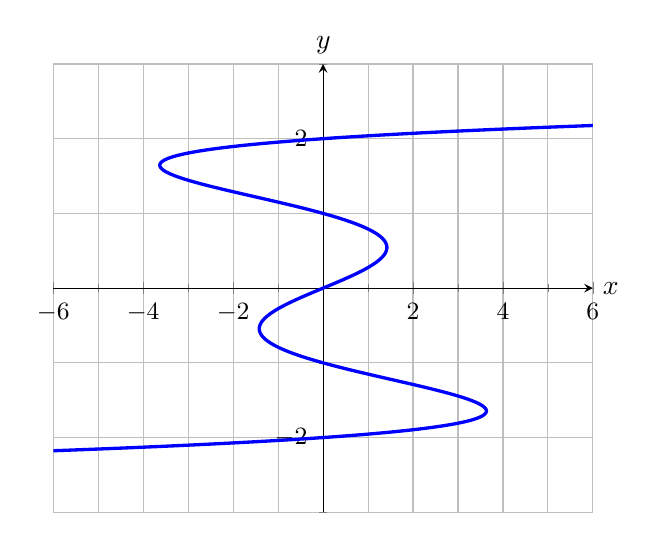
\begin{tikzpicture}
  \begin{axis}[
    axis lines=middle,
    xlabel={$x$},
    ylabel={$y$},
    xmin=-6, xmax=6,
    ymin=-3, ymax=3,
    grid=both,
    minor tick num=1,
    enlargelimits=false,
    ticklabel style={font=\small},
    every axis x label/.style={at={(current axis.right of origin)}, anchor=west},
    every axis y label/.style={at={(current axis.above origin)}, anchor=south},
  ]

    % Parametric plot: t plays the role of y
    % (x(t), y(t)) = (t^5 - 5 t^3 + 4 t, t)
    \addplot[
      domain=-2.5:2.5,  % extend if you want to see more of the curve
      samples=500,
      very thick,
      blue
    ] ({x^5 - 5*x^3 + 4*x}, {x});

  \end{axis}
\end{tikzpicture}
With your group, explain how you would answer the following questions using both the symbolic equation and the curve graph.
  \begin{enumerate}
    \item Is it possible to express $y$ as an explicit function of $x$? 
        \begin{enumerate}
            \item Explain your reasoning using the graph.
            \item Explain your reasoning using the symbolic equation for the curve 
        \end{enumerate}
  \end{enumerate}
\end{exercise}





\end{document}
